\documentclass{beamer}
\usepackage[utf8]{inputenc}
\usepackage[frenchb]{babel}
\usepackage[T1]{fontenc}

\usetheme{Warsaw}

\title[Rapport final de GRO]
      {Rapport final du projet de\\Graphes et Recherche opérationnelle}
\institute{Enseeiht}
\author
  [Ahlouche \and Arthaud \and Auguste
    \and Carton \and Forgione \and Wagner]
  {Maxence Ahlouche \and Maxime Arthaud \and Korantin Auguste
    \and Martin Carton \and Thomas Forgione \and Thomas Wagner}
\date{17 décembre 2013}

\begin{document}

\begin{frame}
  \titlepage
\end{frame}

\begin{frame}{Introduction}
  Blabla
\end{frame}

\section{Jeux}

\begin{frame}{Shifumi}
    \begin{block}{Équilibre de Nash}
        Équilibre de Nash~: jouer de manière aléatoire.
    \end{block}

    \begin{itemize}
        \item Chaines de Markov~: bat aisément un humain qui joue «~normalement~».
        \item Variantes~: reviennent au Shifumi classique si le nombre d'éléments est impair.
    \end{itemize}
\end{frame}

\section{Graphes}

\begin{frame}{Voyageur de commerce}
\end{frame}

\begin{frame}{Énoncé}
    Chercher un chemin passant par tous les sommets, de longueur minimale.
    \begin{itemize}
        \item cycle hamiltonien de coût minimal
        \item NP-complet
        \item méthodes approchées
    \end{itemize}
\end{frame}

\begin{frame}{Résolution approchée}
    \begin{block}{Heuristiques}
        Aller sur le nœud le plus près
    \end{block}

    \begin{block}{Recherche locale}
        \centering
        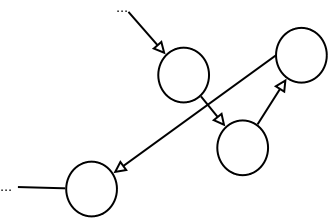
\includegraphics[width=0.3\textwidth]{../rapport/graphes/2opt1.png}
        ~~~~ % j'ai honte, martin help !
        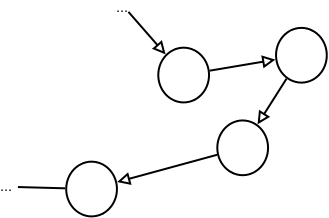
\includegraphics[width=0.3\textwidth]{../rapport/graphes/2opt2.png}
    \end{block}
\end{frame}

\begin{frame}{Métaheuristiques}
    \begin{itemize}
        \item Recherche locale itérée
        \item Recherche tabou
        \item Recuit simulé
        \item Algorithmes génétiques
        \item Colonies de fourmis
    \end{itemize}
\end{frame}

\end{document}
